% chap4.tex (Definitions and Theorem)

\chapter{Model, Dataset, and Final Pipeline Description}
\section{Layer Descriptions}
\subsection{Embedding Layer}\label{embeddinglayer}
An \textbf{embedding layer} maps an word index, or integer, into its corresponding embedding.
This layer is usually the first layer in a neural network that processes input such as text.
Given input text $s$, this layer receives as input a sequence of word indexes $BoW(\bm{s})=$ $\bm{x} = x_1,...,x_k$
and maps each word into an embedding.
Thus, for an input text $\bm{s}$, we transform it into a sequence of integers $\bm{x}$, and from there into $\mathbf{E} \in \mathbb{R}^{n \times d}$, where $d$ is
the embedding size. These embeddings are further fine-tuned during training. Because of the large number of
parameters in this layer (number of words allowed times embedding size), it is usually a good idea to
use $L_2$ regularization or dropout in order to avoid or mitigate overfitting.

\begin{figure}[H]
\caption{Visualization of an embedding layer. Word indexes are mapped to word embeddings. This
layer outputs a matrix comprised of stacked embeddings, one for each index.}
\centering
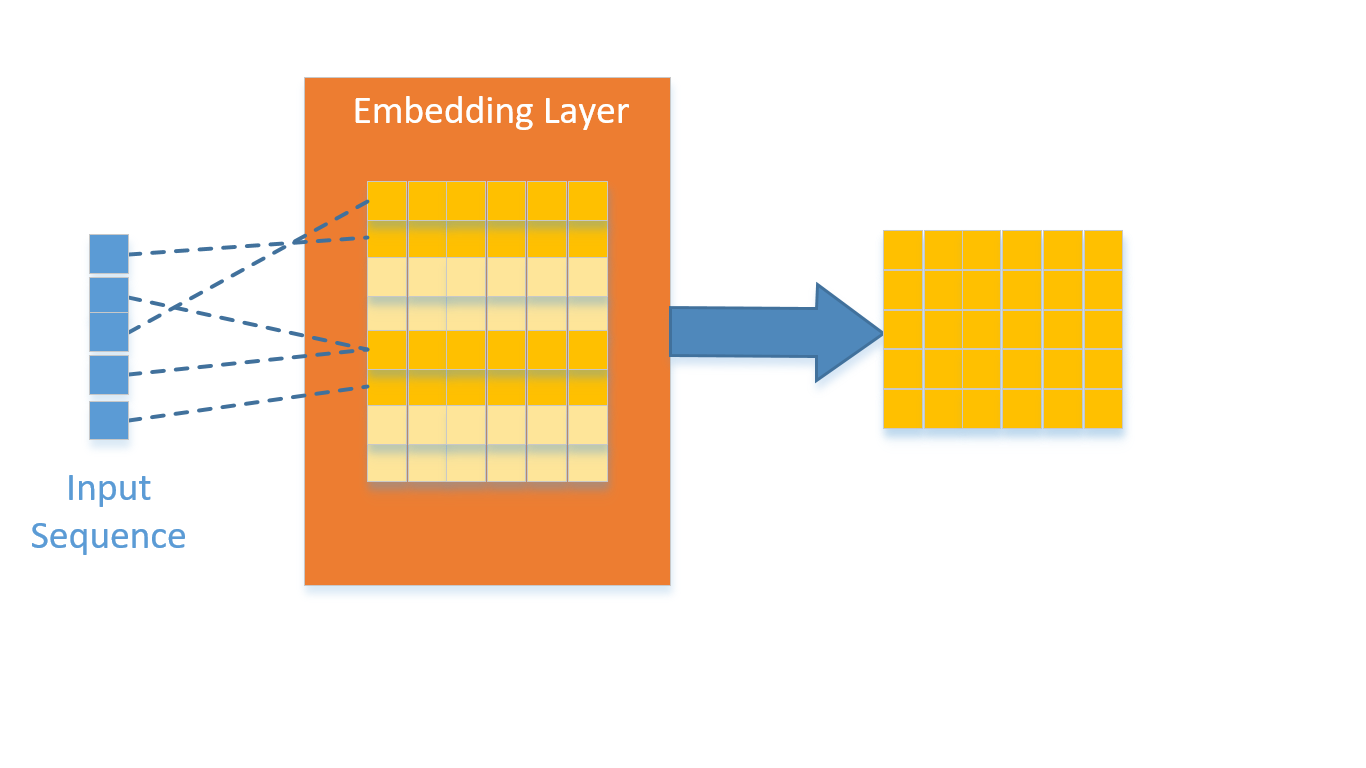
\includegraphics[width=0.5\textwidth]{EmbeddingLayer.png}
\end{figure}

\subsection{Feature Maps: Convolution + Pooling}

We refer to a convolutional layer followed by a pooling layer as a feature map.
Since our data are text sequences and thus have temporal structure, we use a one-dimensional convolutional
layer to convolve with embedding n-grams through the input sequence \cite{waibel1988phoneme}.
As in Figure \ref{fig:convolution}, we stride only along the time dimension. This is in contrast to the usual two-dimensional convolution schemes with image data,
where the kernels stride along the width and height dimensions of the input data. After the convolution step,
we apply a non-linearity to each computed feature. We chose the rectified linear activation (\textbf{ReLU}) function
\[ReLU(x) = max(0,x)\]
Although simple, this non-linearity is quite effective and thus widely used.
We then use a max pooling operation to ouput a single value for each kernel similar to \cite{DBLP:journals/corr/LinCY13}. Besides the huge
dimensionality reduction, we do this so that we pass to the next layer the single strongest activation
from each kernel i.e. a strong feature selection mechanism.

\subsection{Gated Recurrent Unit Layer}
A recurrent layer is designed to process data with temporal structure i.e. sequences \cite{rumelhart1986sequential}.
This recurrent layer is in itself a network, where the hidden layer values at time \textit{t} depend on the previous
hidden layer's values, the input corresponding to time \textit{t}, and a shared parameter set:
\[\bm{h}^{t} = f(\bm{h}^{t-1}, \bm{x}^{t}, \bm{\theta})\]
This is implemented by \textit{unrolling} the layer along the time dimension as a sequence of layers, each corresponding
to the next in time. Because of this design, back propagation of error through the unrolled layer can result
in the vanishing gradient problem.

\begin{figure}[H]
\caption{Visualization of a recurrent layer. Each hidden layer $\bm{h}^{\textit{t}}$ is a function of the previous hidden
layer $\bm{h}^{\textit{t-1}}$, the present input signal $\bm{x}^{\textit{t}}$. The weights are shared across time steps
in order for the model to generalize better.}
\centering
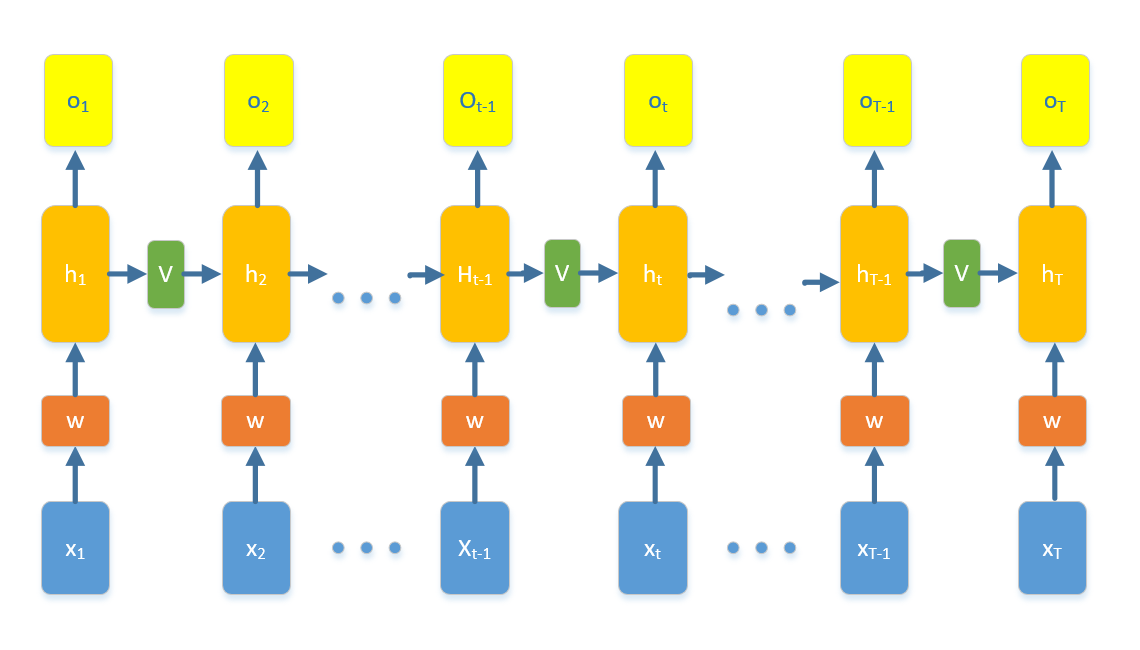
\includegraphics[width=0.5\textwidth]{RecurrentNet.png}
\end{figure}

A Gated Recurrent Unit layer is a type of recurrent layer designed to combat this condition \cite{chung2014empirical}.
It is a simplified version of the earlier LSTM layer \cite{hochreiter1997long}, also designed to mitigate the vanishing gradient problem,
and in practice it performs comparably well.
This layer models the latent features computed by the feature map as a time sequence. This means that it
does not assume indepences between activation and learn to model the temporal structure of the previous
layer's output. This property makes the layer an adequate choice, since we deal with text data which inhibits
temporal structure.

\subsection{Dense Layer}
The last layer in our model is the classical \textbf{dense}, or fully connected layer.
The number of units in this layer is equal to the number of classes in our dataset.
Given the output of the network's second to last layer $\bm{h}$, we can compute the unnormalized log probabilities
\[\bm{z} = \bm{W}^{T}\bm{h} + \bm{b}\]
for some bias vector $\bm{b}$.



Each  $z_i$ is a log probability of the input corresponding to class $i$. The \textbf{softmax} activation function is then applied to
the all units, to finally output class probabilities:

\[\hat{y}_i = softmax(\bm{z})_i = \frac{exp(z_i)}{\sum_j exp(z_j)}\],
\[\hat{y}_i = P\{y=i|\bm{x}\}\]

\section{Model Description}

\cite{yin2017comparative} provide an overview of typical neural models used for natural language processing.
A standard architecture for convolutional neural networks for text sequence classification is the one proposed by
\cite{kim2014convolutional}. This model has an embedding layer followed by a feature map and a dense layer with a softmax activation
to output class probabilities. This model has parameter sharing and sparse interaction properties inherent of convolutional
neural networks, and thus is a good choice for efficiently extracting features from the data via convolutions and non-linearities.
The pooling operation provides data dimensionality and acts as a translation invariance mechanism. This reduction makes forward propagation
an even more efficient process. Convolutional neural networks, however, are not designed to consider the data as having temporal
structure, as is the case with text sequence data.

Another popular neural model for text classification is the recurrent neural network. This architecture is explicitly designed to treat
data to display temporal structure. Because of this, the recurrent neural network is an excelent choice for text sequence data.
At a basic level, this architecture is comprised of an embedding layer (to transform input sequences into word embeddings)
followed by a recurrent layer e.g. LSTM or GRU, then a dense layer with the softmax activation to output probabilities.

In our experiments, a purely convolutional neural network displayed great efficiency relative to the recurrent network. Because of the convolution
and pooling operations, the CNN normally processed the data around 10 times as fast as the RNN. The RNN, although slower,
always achieved around 4\% higher accuracy on all experiments, due perhaps to its ability to model sequential data.

After testing both architectures, the model we use in the rest of this work is a mixture of these two standards.
After the embedding layer, we add a feature map to extract features from the raw inputs,
then we add a GRU layer. This design choice incorporates the sequence modeling power of the RNN with the fast and efficient feature extraction of the CNN.
This combination always led to the higher accuracy achieved with the RNN, with training times orders of magnitude shorter as with the CNN.
We further extended our pooling operation to be global. Out of all the features computed by a kernel, we select only the single strongest one
(i.e. highest value). The pooling layer's output size is therefore equal to the number of kernels in our convolutional layer. In order to create
a one-to-one correspondance between the network's inputs (the word indices in the input sequence) and the units in the recurrent layer, we chose to have
a number of kernels equal to the network's input size (i.e. length of input sequence).
This design choice proved to be very efficient and reached the highest accuracy percentages during our experiments.

\begin{figure}[H]
\caption{Model Architecture: embedding layer, followed by a feature map, and a recurrent layer. At the end, we have
a fully connected layer with a softmax activation, which will output class probabilities.}
\centering
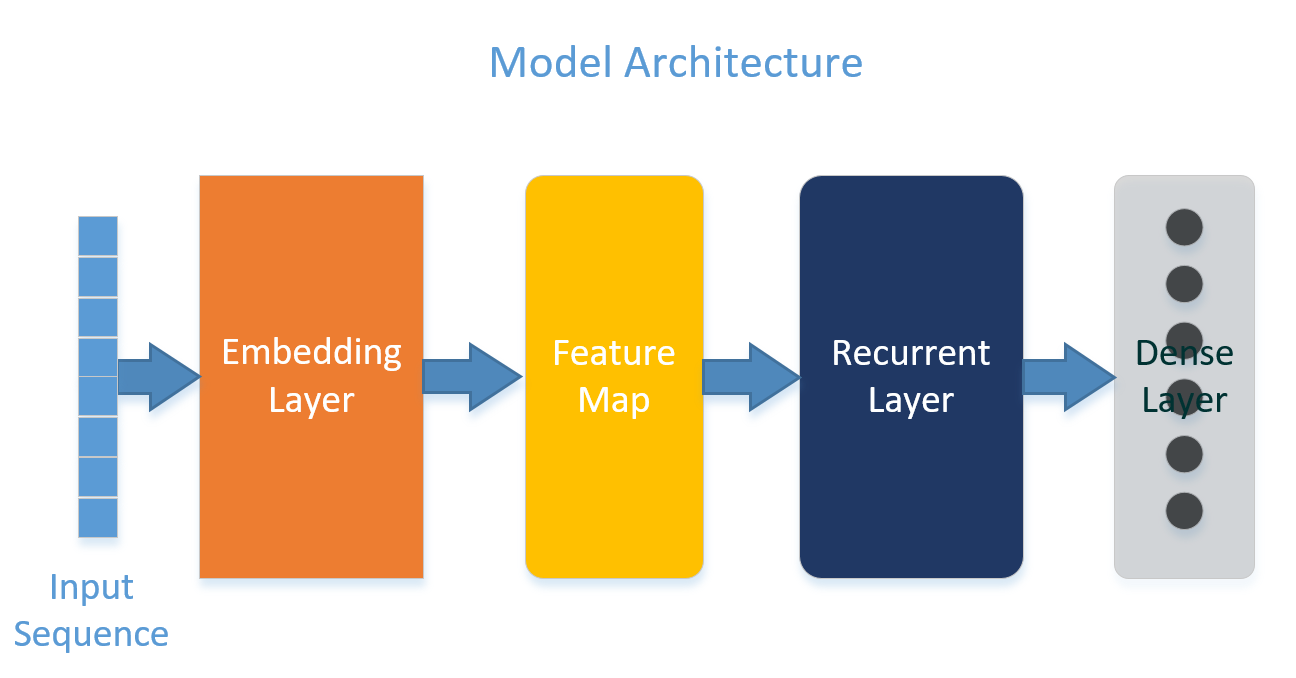
\includegraphics[width=0.5\textwidth]{ModelPipeline.png}
\end{figure}

The final network's architecture is as follows:
\begin{itemize}
  \item Input layer: word index vector
  \item Embedding layer: maps word index vector to embedding matrix
  \item Feature Map:
      \begin{itemize}
        \item Convolution layer: kernel size=5, \textit{ReLU} activation
        \item Global MaxPooling layer: Outputs a scalar per kernel
      \end{itemize}
\item Gated Recurrent Unit layer with \textit{tanh} activations
\item Dense layer with \textit{softmax} activations
\end{itemize}
